\chapter{Planos Técnicos}

\begin{figure}[H]
	\centering
	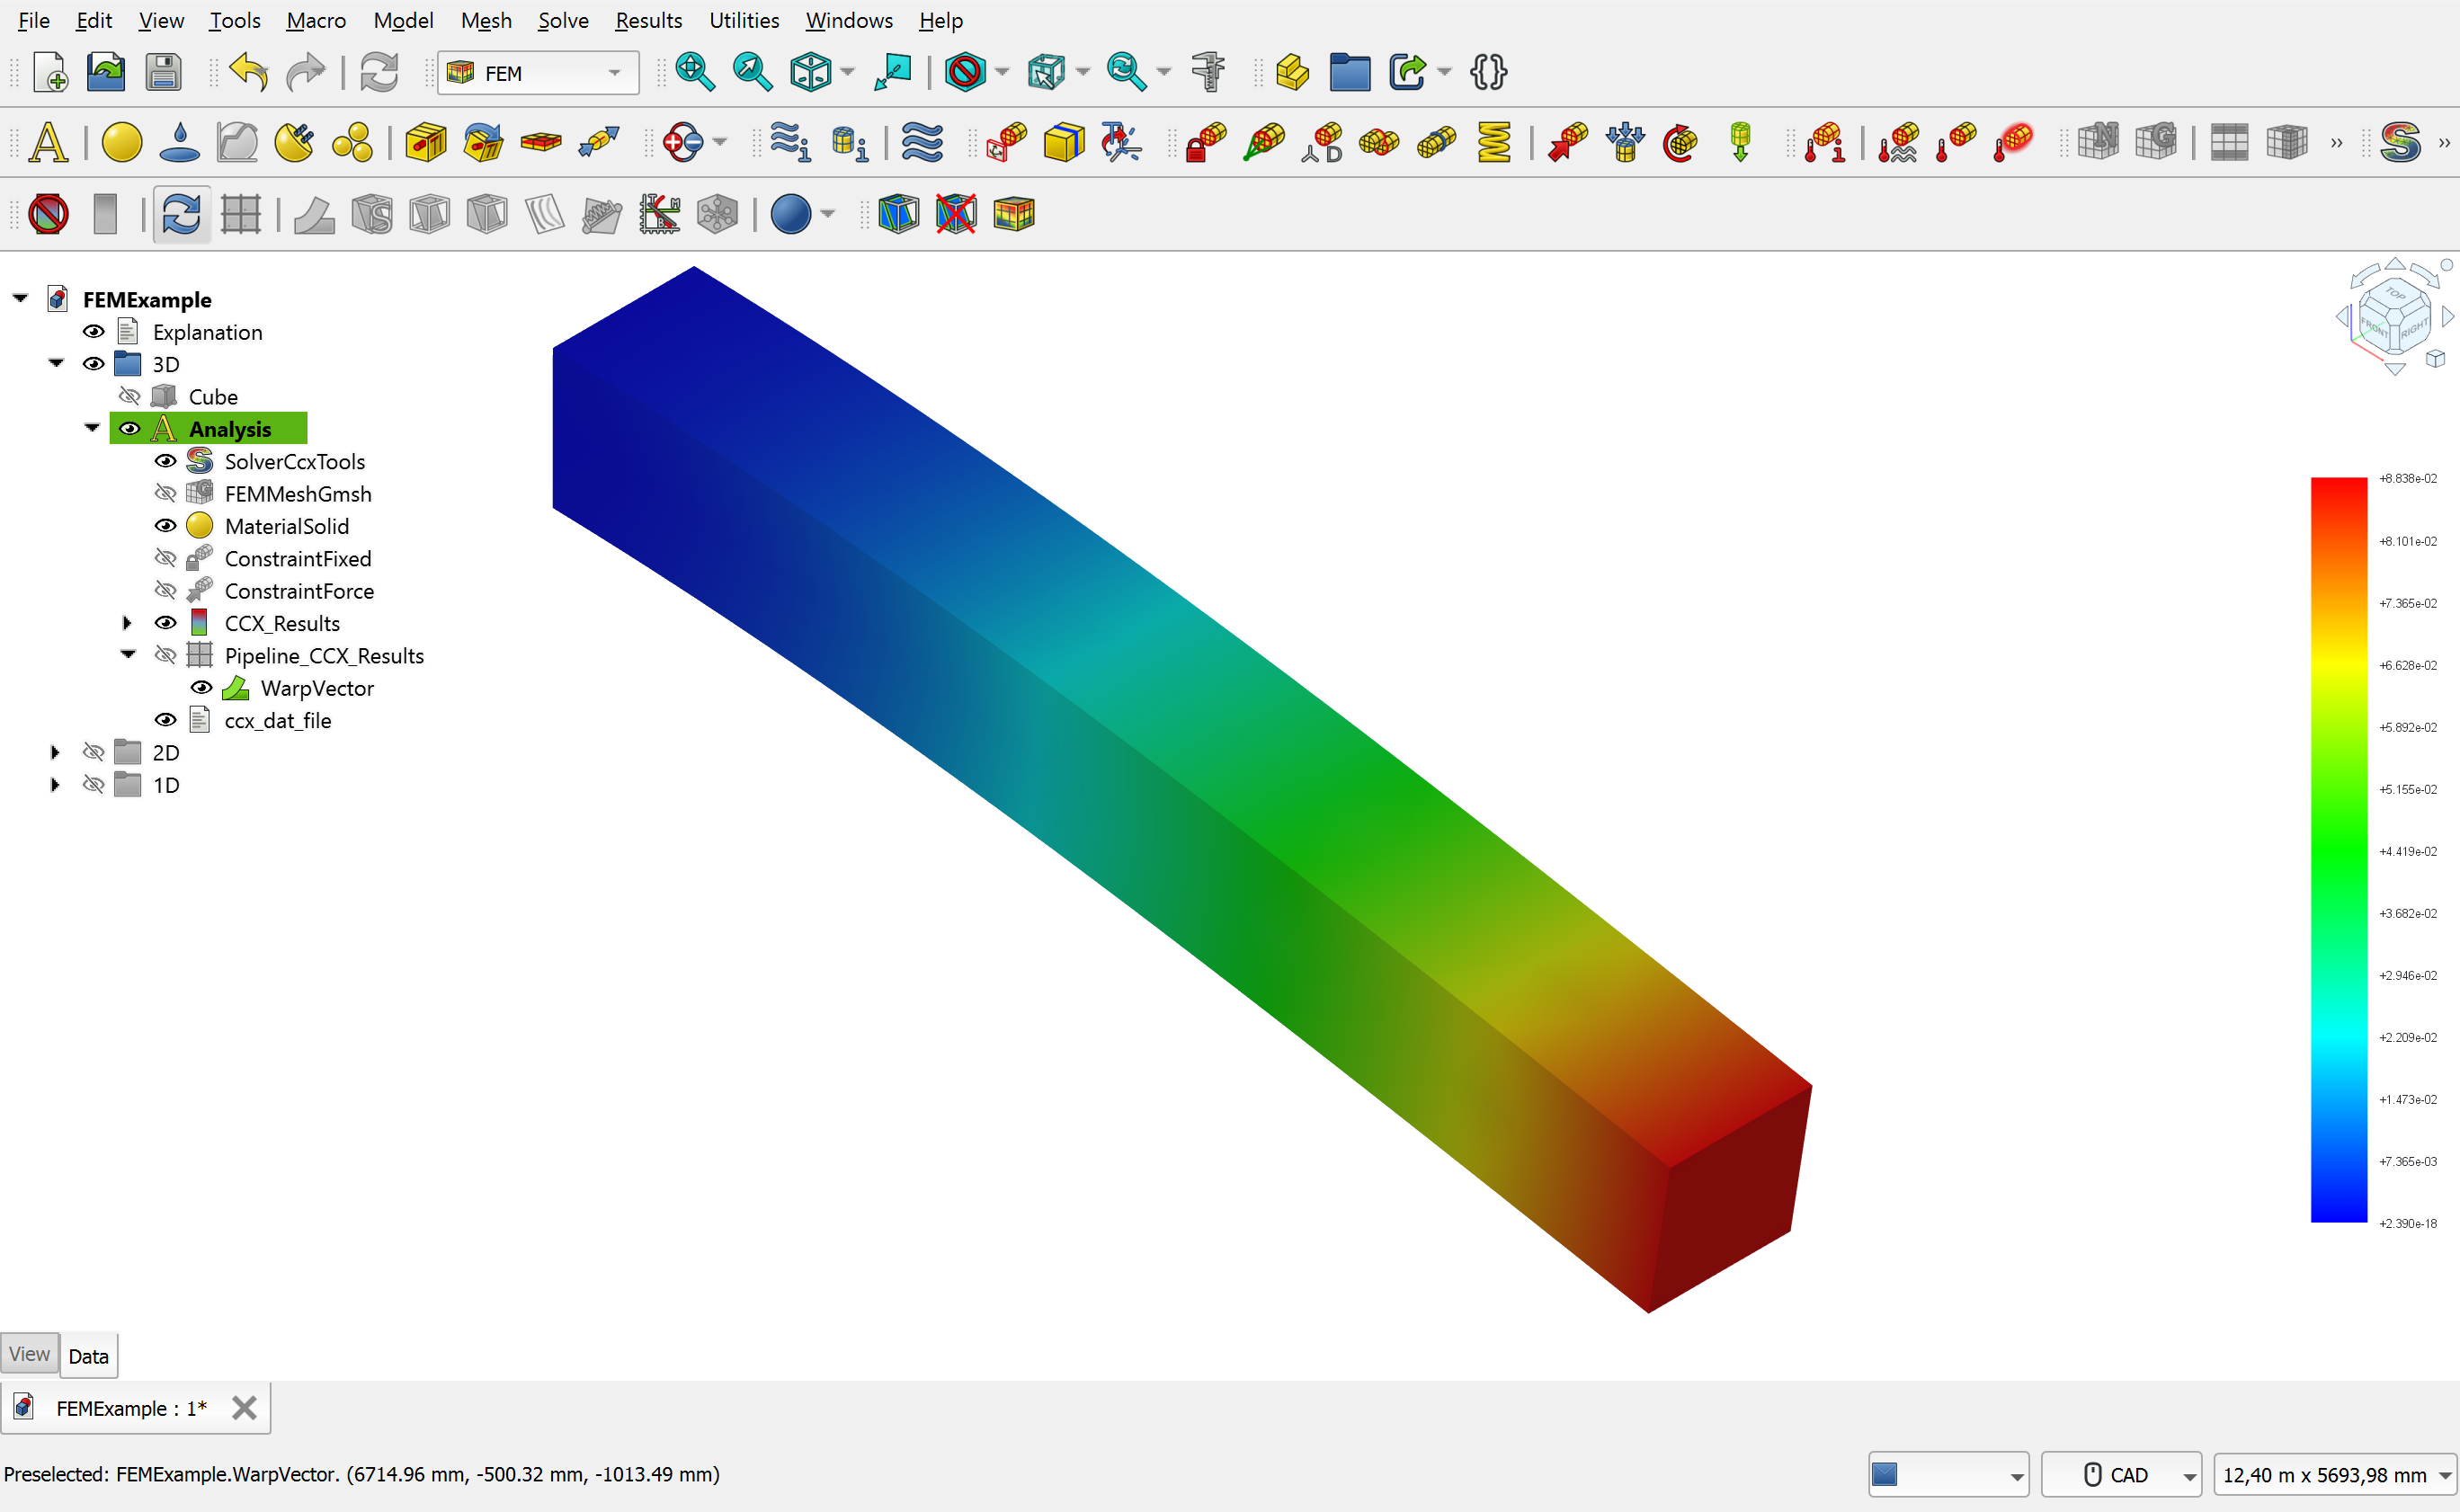
\includegraphics[width=0.8\textwidth]{img/cap8_planos.png}
	\caption{Plano técnico generado con el módulo TechDraw}
\end{figure}

Aprende a crear planos técnicos profesionales con
FreeCAD. Genera documentación técnica a partir de
modelos 3D usando el módulo TechDraw.

%% D. Búsqueda e Inserción de Activos Gráficos
%% Imagen insertada al inicio del capítulo

%% B. Actividades Teóricas
\section{Investigar y responder}
\faPencil

Investiga sobre planos técnicos en FreeCAD y responde:
\begin{enumerate}
	\item ¿Qué es un plano técnico y para qué sirve?
	\item ¿Cuáles son las vistas principales en un plano?
	\item ¿Cómo se generan vistas ortográficas desde un
	      modelo 3D?
	\item ¿Qué son las cotas de referencia y de cota?
	\item ¿Cómo se añaden anotaciones y símbolos a un plano?
	\item ¿Qué formatos de exportación soporta TechDraw?
	\item ¿Cómo se personalizan los estilos de plano?
	\item ¿Qué normas técnicas se deben seguir en planos?
\end{enumerate}

%% C. Actividades Prácticas
\section{Resolver los siguientes problemas}
\faWrench

Problemas para aplicar conocimientos:
\begin{enumerate}
	\item Abre un modelo 3D existente en FreeCAD.
	\item Crea un nuevo plano usando el módulo TechDraw.
	\item Añade una vista frontal del modelo al plano.
	\item Añade vistas lateral y superior del modelo.
	\item Inserta cotas dimensionales en el plano.
	\item Añade una vista isométrica del modelo.
	\item Incluye leyenda y título en el plano.
	\item Exporta el plano a formato PDF.
	\item Personaliza los estilos de líneas y cotas.
	\item Crea un plano completo con todas las vistas
	      necesarias para fabricación.
\end{enumerate}